
\subsection{John Backus and Fortran}

IBM did not feel that Aiken and the Harvard Computation Laboratory had given
them sufficient credit for their contributions to the Mark I, which left
Thomas Watson Sr. and the IBM folks bitter about the experience and eager to
produce a new device entirely in-house. This device would become the Selective
Sequence Electronic Calculator, or the SSEC. It was built on 57th Street in
Manhattan, and it was monstrous. Roughly 50 by 100 feet with a giant console
and hundreds of toggle switches and tape units and relays behind glass panels;
there were giant windows that allowed passersby to see the machine in action.

One such passerby was John Backus, a recent Masters graduate from Columbia
University. He was intrigued by the machine, which he mentioned to his tour
guide, who suggested he go upstairs and talk to the boss about it. Robert "Rex"
Seeber gave him a puzzle, which he solved, and he was hired on the spot
\cite{backus_oral_history_2006}.

In 1942, Backus majored in Chemistry at the University of Virginia where he
struggled academically. He was expelled due to poor attendance within the first
year before being drafted into the US Army. He commanded an antiaircraft
battery at Fort Steward, Georgia, remaining in the US for the remainder of
WWII.

While he did not at first find success in academia, he got very good marks on
military aptitude tests. He was directed to the University of Pittsburgh's
engineering program and later to a premedical program at Haverford College near
Philadelphia (which is where he grew up). In 1945 he attended the Flower and
Fifth Avenue Medical School in NYC, but he was still struggling with the
academy. He was uninterested in medicine, feeling that it was all about
memorization. He dropped out after less than a year.

He entered a radio technician school and became interested in math, which led
him to enroll in the math program at Columbia University. The SSEC that would
intrigue him at the IBM computing center was designed at the Watson Scientific
Computing Laboratory at Columbia.

\subsection{Speedcoding to FORTRAN}

At IBM, Backus worked on the SSEC and later the IBM 701 and 704. The main use
of the SSEC was aerospace calculations; programming calculations to predict the
position of the moon was one of the first tasks he was given at IBM. He would
continue writing programs for these machines in spite of their poor usability.
His team's techniques would be used in the lunar missions of the 1960s.

The pain of writing programs for these early machines entirely in machine code
drove him to explore new ways to program. The first of these was a symbolic
notation for floating point arithmetic and address expression calculation
called Speedcoding\cite{backus_oral_history_2006}:

\begin{quotation}
	\textbf{Grady Booch:}
	So then from your experience with the SSEC, you then went on to
	produce Speedcoding, the
	Speedcoder\dots
	What were sort of the things that influenced you to create that in
	the first place?

	\textbf{John Backus:}
	Well, programming in machine code was a pretty lousy business to
	engage in, trying to figure
	out how to do stuff. I mean, all that was available was a sort of a
	very crude assembly program. So I
	figured, well, let's make it a little easier. I mean it was a
	rotten design, if I may say so, but it was better
	than coding in machine language.
\end{quotation}

The IBM 701 did not have an index register, so calculating addresses for array
operations was tedious and error-prone. Speedcoding provided a way to express
these calculations symbolically.

\begin{figure}[h!]
	\centering
	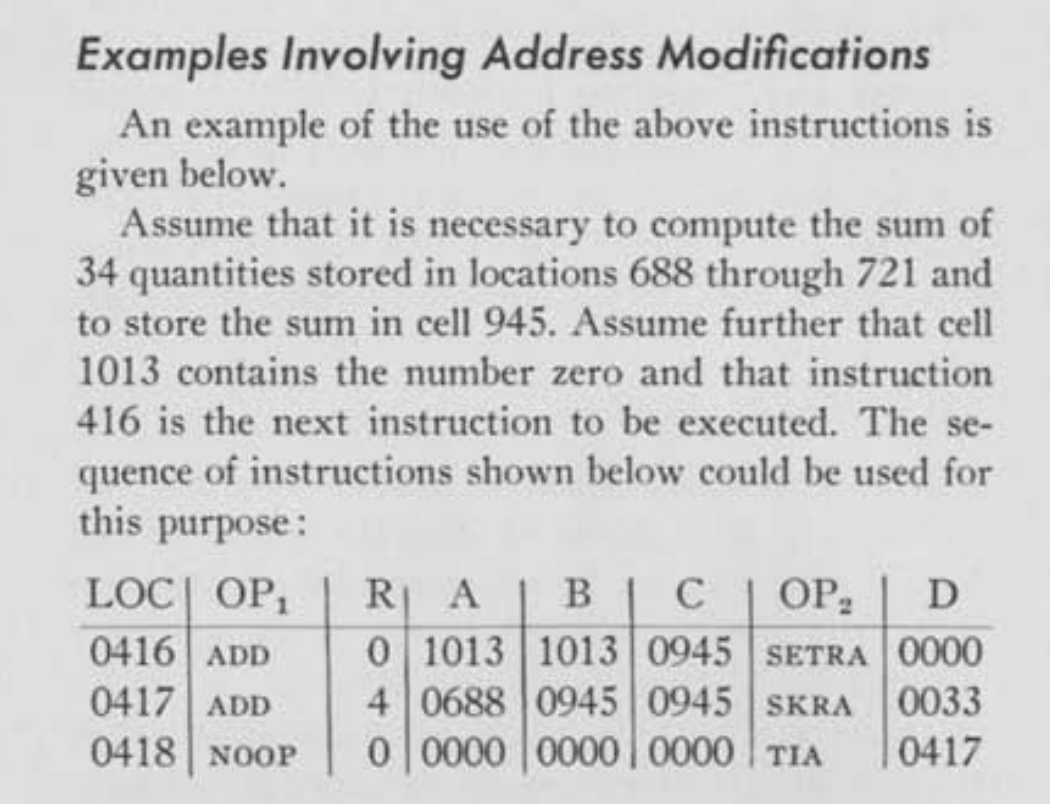
\includegraphics[width=0.5\linewidth]{resource/ibm-speedcoding-example.png}
	\caption{Excerpt from \textit{IBM Speedcoding for the Type 701
			Electronic Data Processing Machine}
		\cite{IBM_1954_Speedcoding}}
	\label{fig:ibm-speedcoding-example}
\end{figure}

The 704 was the first machine to have such a register; it also had floating
point instructions and core memory, more or less obviating the need for
Speedcoding: "we were moving to the 704, which had built in floating point,
built in index registers, which was all that Speedcoding was supposed to
supply. So what the hell?" \cite{backus_oral_history_2006} He credits himself
with getting index registers and floating point into the 704.

%Here is an example from the IBM Speedcode manual\cite{IBM_1954_Speedcoding}:
%\begin{quotation}
%    Assume that it is necessary to compute the sum of 34 quantities stored in
%    locations 688 through 721 and to store the sum in cell 945.
% Assume further that
%    cell 1013 contains the number zero and that instruction 416 is the next
%    instruction to be executed. The sequence of instructions shown
% below could be
%    used for this purpose:
%
%    \begin{center}
%    \begin{tabular}{cccccccc}
%    \hline
%    LOC & OP$_1$ & R & A & B & C & OP$_2$ & D \\
%    \hline
%    0416 & ADD  & 0 & 1013 & 1013 & 0945 & SETRA & 0000 \\
%    0417 & ADD  & 4 & 0688 & 0945 & 0945 & SKRA  & 0033 \\
%    0418 & NOOP & 0 & 0000 & 0000 & 0000 & TIA   & 0417 \\
%    \hline
%    \end{tabular}
%    \end{center}
%\end{quotation}

Backus did not think all that highly of Speedcoding in retrospect, though it
gained traction in large part due to IBM's marketing power and the number of
users of the 701 relative to the size of the computer market at the time
\cite{Backus_1980_Programming_in_America_in_1950s}. It is unclear whether
Backus's assessment of his own code is accurate or if it's born of humility.

\begin{quotation}
	The success of some programming systems depended on the number of machines
	they would run on. Thus, an elegant system for a one-of-a-kind machine might
	remain obscure while a less-than-elegant one for a production
	computer achieved popularity.

	This point is illustrated by two papers at the 1954 ONR symposium
	One, by David E. Muller, describes a floating point interpretive system for
	the ILLIAC designed by D. J. Wheeler. The other, by Harlan Herrick and myself,
	describes a similar kind of system for the IBM 701 called Speedcoding. Even
	today Wheeler's 1954 design looks spare, elegant, and powerful, whereas the
	design of Speedcoding now appears to be a curious jumble of compromises.
	Nevertheless, Wheeler's elegant system remained relatively obscure (since only
	ILLIAC users could use it) while Speedcoding provided enough conveniences,
	however clumsily, to achieve rather widespread use in many of the eighteen 701
	installations.
\end{quotation}

In 1953, based on his experience with Speedcoding on the 701, Backus proposed
yet another language to elevate the programming experience on the 704. IBM
management supported the proposal. He formed a ten-person team of his own
choosing based out of IBM's Manhattan headquarters, including Irving Ziller,
\todo{list other members}. They released \citetitlecite{IBM_1954_FORTRAN_Specifications}
after about one year of working
together.
Roughly two years after its first conception, \FTN{} was released for
the first time. It would go on to ship with every IBM 704 and become the
primary means of programming in the scientific community.

Backus could not
stand how slow programming was without a higher-level language, and machines
were expensive; leasing a machine and spending time programming in machine code
wasted money compared to a compiler capable of generating reasonable machine
code (though at the time it usually underperformed hand-written code). Backus
and his team would continue to develop and stabilize this compiler for several
years, though.

\begin{quotation}
	\FTN{} did not really grow out of some brainstorm about the beauty of
	programming in mathematical notation; instead it began with the recognition
	of a basic problem of economics: programming and debugging costs already
	exceeded the cost of running a program, and as computers became faster
	and cheaper this imbalance would become more and more intolerable. This
	prosaic economic insight, plus experience with the drudgery of coding, plus
	an unusually lazy nature led to my continuing interest in making
	programming easier.
	This interest led directly to work on Speedcoding for the 701
	and to efforts to have floating point as well as indexing built into the 704.
	\cite{Backus_1980_Programming_in_America_in_1950s}
\end{quotation}

When Backus was forming his team in January of 1954, he was moved from the Pure
Science department at IBM into the Applied Science department because his boss
Rex Seeber wanted nothing to do with the project. There he found Irving Ziller,
who became his first teammate. By April, they had been joined by Harlan Herrick
who co-authored the Speedcoding paper with Backus at the ONR symposium
\citetitle{Backus_Herrick_1954_Speedcoding} in which they observe:

\begin{quotation}
	The question is, can a machine translate a sufficiently rich mathematical
	language into a sufficiently economical program at a sufficiently low cost to
	make the whole affair feasible?  consider the advantages of being
	able to state
	the calculations\dots for a problem solution in a concise, fairly natural
	mathematical language.
\end{quotation}

The reader should note that it is often incorrectly asserted (at times even by
Backus himself\cite{Backus_1980_Programming_in_America_in_1950s}) that this
came \textit{after} Backus and Ziller had been given a demonstration of Laning
and Zierler's algebraic compiler for the Whirlwind at MIT at the ONR symposium
of 1954. When they received this demonstration, there were already four members
of the \FTN{} team, Irving Ziller, Robert Nelson, Harlan Herrick, and Backus
himself. In Backus's words\cite{Backus_1980_Programming_in_America_in_1950s}:

\begin{quotation}
	The article and the letter therefore show that, much to my surprise, the
	FORTRAN effort was well under way before the ONR symposium and that,
	independently of Laning (but later), we had already formulated more ambitious
	plans for algebraic notation (e.g., Gail bjk) than we were later to find in
	Laning and Zierler's report and see demonstrated at MIT. It is therefore
	unclear what we learned from seeing their pioneering work, despite my mistaken
	assumption over the years that we had gotten our basic ideas from them
\end{quotation}

Indeed, even Grace Hopper made the same assertion at a 1956 symposium:

\begin{quotation}
	A description of Laming and Zierler' s system of algebraic pseudocoding for
	the Whirlwind computer led to the development of Boeing 's BACAIC for the 701,
	FORTRAN for the 704, AT-3 for the Univac, and the Purdue System for the Datotron and
	indicated the need for far more effort in the area of algebraic
	translators.
	\cite{Knuth_TrabbPardo_1976_Early_Development}
\end{quotation}

Donald Knuth and Trabb Pardo quote her in \citetitle{Knuth_TrabbPardo_1976_Early_Development}
as well.
I am not sure who to believe either!

With the support of his new boss Cuthbert Hurd, his family, friends, and his
team, the first report of \FTN{} was released externally to 704 users. This
brought interest from a variety of users, many of whom offered up members of
their teams to help.

The original FORTRAN report had some peculiarities and made some large claims,
some of which came true and some of which \textit{very much} did not.
Variables had one or two characters, function names of three or more characters,
and array variables with up to three subscripts.
The document used the term \textit{arithmetic formulas} to describe what
we would today call \textit{assignment statements}.

\begin{figure}[h!]
	\centering
	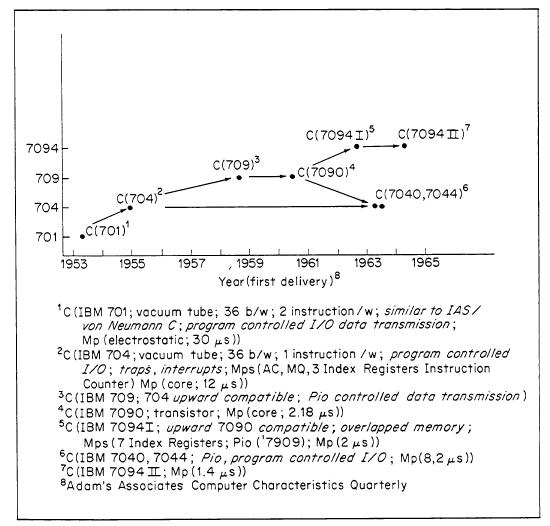
\includegraphics[width=0.5\linewidth]{resource/ibm-7094.jpeg}
	\caption{Excerpt from \textit{The IBM 701--7094 II Sequence: A
			Family by Evolution}
		\cite{Hamming_Feigenbaum_1971_IBM7094}, illustrating the
		instruction structure for summing quantities.}
	\label{fig:ibm7094-example}
\end{figure}

DO formulas were particularly interesting, and not necessarily the construct that we
today call \textit{loops}.
Any \textit{formula} could have an associated number with it, allowing that formula to be
invoked from elsewhere in the program.
For example, in the following snippet taken from the original report,
the formulas starting with 10 and ending with 14 would be executed
9 times in total, starting with i taking the value of 4 and incrementing by 2
until reaching 20; once completed, control resumes at formula 30:

\begin{lstlisting}[language=fortran,frame=single]
      do 10 14 30 i=4,20,2
\end{lstlisting}

Whew! For such a fundamental concept, the \gls{cfg} is potentially very complex.
I suspect that in most cases, only one or two formulas were specified.
When the third formula number is omitted, execution resumes at the instruction
immediately following the final formula of the DO construct, and
if only one formula is specified, then that is the last formula to execute,
and the first is the one immediately following the DO statement.

Another peculiar feature was the RELABEL formula, which was intended to make
matrix rotation operations simpler. For example, for a 4x4 matrix \texttt{b}, the
formula \texttt{RELABEL(3,1)} would result in \texttt{b(1,i)} taking the same meaning as \texttt{b(i,1)}
had prior to the relabel.
There soon came better ways to express the same idea, and I am unable to find any example
programs using this construct, even in the original report.

The final section of the report notes that "no special provisions have been included
in the FORTRAN system for locating errors in formulas\dots
Since FORTRAN formulas are fairly readable, it should be possible to
check their correctness by independently recreating the specifications for
the problem from its FORTRAN formulation." \cite[C. DEBUGGING]{IBM_1954_FORTRAN_Specifications}
It is remarkable that they \textit{did} consider how to debug FORTRAN programs,
and then \textit{thought better} of providing error messages.

Again, they were tragically optimistic: in the second page of the report,
they claimed that "FORTRAN should virtually eliminate coding and debugging."
